\section{Anforderungsanalyse}

\begin{concept}{Übersicht Anforderungsanalyse}
\begin{itemize}
    \item Anforderungen sind nie vollständig im Voraus bekannt
    \item Entwickeln sich während des Projekts
    \item Müssen mit Stakeholdern erarbeitet werden
    \item "I don't know what I want but I'll tell you when I see it!"
\end{itemize}
\end{concept}

\subsubsection{Usability und User Experience}

\begin{concept}{Usability und User Experience}
Die drei Säulen der Benutzererfahrung:
\begin{itemize}
    \item \textbf{Usability (Gebrauchstauglichkeit):} Grundlegende Nutzbarkeit des Systems
    \item \textbf{User Experience:} Usability + Desirability (Attraktivität)
    \item \textbf{Customer Experience:} UX + Brand Experience (Markenwahrnehmung)
\end{itemize}
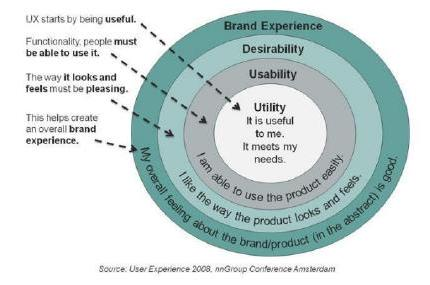
\includegraphics[width=0.9\linewidth]{images/2024_12_29_0d1d7b5551ea1b4b41bdg-02}
\end{concept}

\begin{KR}{Erfassen von Usability-Anforderungen}
\begin{enumerate}
    \item Nutzergruppen identifizieren
    \begin{itemize}
        \item Primäre Nutzer
        \item Gelegentliche Nutzer
        \item Systemadministratoren
    \end{itemize}
    \item Nutzungskontext analysieren
    \begin{itemize}
        \item Physische Umgebung
        \item Technische Umgebung
        \item Soziale Umgebung
    \end{itemize}
    \item Messbare Kriterien definieren
    \begin{itemize}
        \item Erfolgsrate bei Aufgaben
        \item Zeitbedarf für Aktionen
        \item Fehlerrate bei Bedienung
    \end{itemize}
\end{enumerate}
\end{KR}

[Previous content for Usability-Dimensionen and ISO 9241-110 remains...]

\begin{example}{Messbare Usability-Kriterien}
Für ein Bankomat-System:
\begin{itemize}
    \item \textbf{Effektivität:} 98\% aller Geldabhebungen erfolgreich
    \item \textbf{Effizienz:} Standardabhebung in max. 30 Sekunden
    \item \textbf{Zufriedenheit:} Mind. 4 von 5 Punkten in Nutzerbefragung
    \item \textbf{Fehlertoleranz:} Max. 1\% Abbrüche durch Bedienfehler
\end{itemize}
\end{example}

[Previous content for User-Centered Design remains...]

\begin{KR}{Erstellen einer Persona}
\begin{enumerate}
    \item Nutzungskontext recherchieren
    \begin{itemize}
        \item Interviews durchführen
        \item Nutzungsverhalten beobachten
        \item Existierende Daten analysieren
    \end{itemize}
    \item Persona definieren
    \begin{itemize}
        \item Name und Foto (fiktiv aber realistisch)
        \item Demografische Daten
        \item Technische Affinität
        \item Ziele und Frustrationen
        \item Typische Verhaltensweisen
    \end{itemize}
    \item Persona validieren
    \begin{itemize}
        \item Mit Stakeholdern abstimmen
        \item Mit realen Nutzerdaten vergleichen
    \end{itemize}
\end{enumerate}
\end{KR}

\subsubsection{Requirements Engineering}

\begin{definition}{Requirements (Anforderungen)}
\begin{itemize}
    \item Funktionale Anforderungen: Was das System tun soll
    \item Nicht-funktionale Anforderungen: Wie das System sein soll
    \item Randbedingungen: Einschränkungen und Vorgaben
    \item Müssen mit allen Stakeholdern erarbeitet werden
    \item Entwickeln sich während des Projekts
\end{itemize}
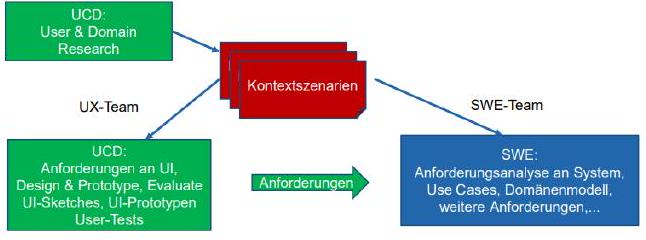
\includegraphics[width=\linewidth]{images/2024_12_29_0d1d7b5551ea1b4b41bdg-04(1)}
\end{definition}

\begin{KR}{Anforderungserhebung}
\begin{enumerate}
    \item Stakeholder identifizieren
    \item Informationsquellen erschließen
    \begin{itemize}
        \item Interviews
        \item Workshops
        \item Beobachtungen
        \item Dokumente
    \end{itemize}
    \item Anforderungen dokumentieren
    \begin{itemize}
        \item Use Cases
        \item User Stories
        \item Szenarien
    \end{itemize}
    \item Anforderungen priorisieren
    \item Anforderungen validieren
\end{enumerate}
\end{KR}

[Previous content for Use Cases section remains...]

\begin{example}{System Sequence Diagram für Bankomat}
\begin{lstlisting}[language=Java]
// Systemoperationen aus SSD
public interface ATMSystem {
    // Kunde authentifizieren
    boolean authenticate(Card card, PIN pin);
    
    // Kontostand abfragen
    Balance getBalance(AccountType type);
    
    // Geldbetrag abheben
    boolean withdraw(Amount amount, AccountType type);
    
    // Beleg drucken
    void printReceipt(Transaction transaction);
}
\end{lstlisting}
\end{example}

\begin{KR}{Prüfung von Use Cases}
Checkliste für qualitativ hochwertige Use Cases:
\begin{enumerate}
    \item \textbf{Vollständigkeit}
    \begin{itemize}
        \item Alle Stakeholder berücksichtigt?
        \item Alle Szenarien abgedeckt?
        \item Vor- und Nachbedingungen definiert?
    \end{itemize}
    \item \textbf{Konsistenz}
    \begin{itemize}
        \item Begriffe einheitlich verwendet?
        \item Keine Widersprüche?
        \item Abstraktionsebene passend?
    \end{itemize}
    \item \textbf{Testbarkeit}
    \begin{itemize}
        \item Eindeutige Erfolgskriterien?
        \item Messbare Eigenschaften?
        \item Nachvollziehbare Abläufe?
    \end{itemize}
\end{enumerate}
\end{KR}

[Your previous example of the library system remains...]